\title{Probabilistic Decoder}

\subsection{Probabilistic Decoder}

A probabilistic decoder is a reinterpretation of model likelihoods
based on coding theory. It is a distribution $p(\mathbf{x}_n\mid \mathbf{z}_n)$  over each value
$\mathbf{x}_n\in\mathbb{R}^D$ given a code $\mathbf{z}_n$. The latent
variables $\mathbf{z}_n$ are interpreted as the hidden representation, or code, of the value
$\mathbf{x}_n$. The decoder is probabilistic because its generated
values (decoding) for any given code is random
\citep{dayan1995helmholtz}.

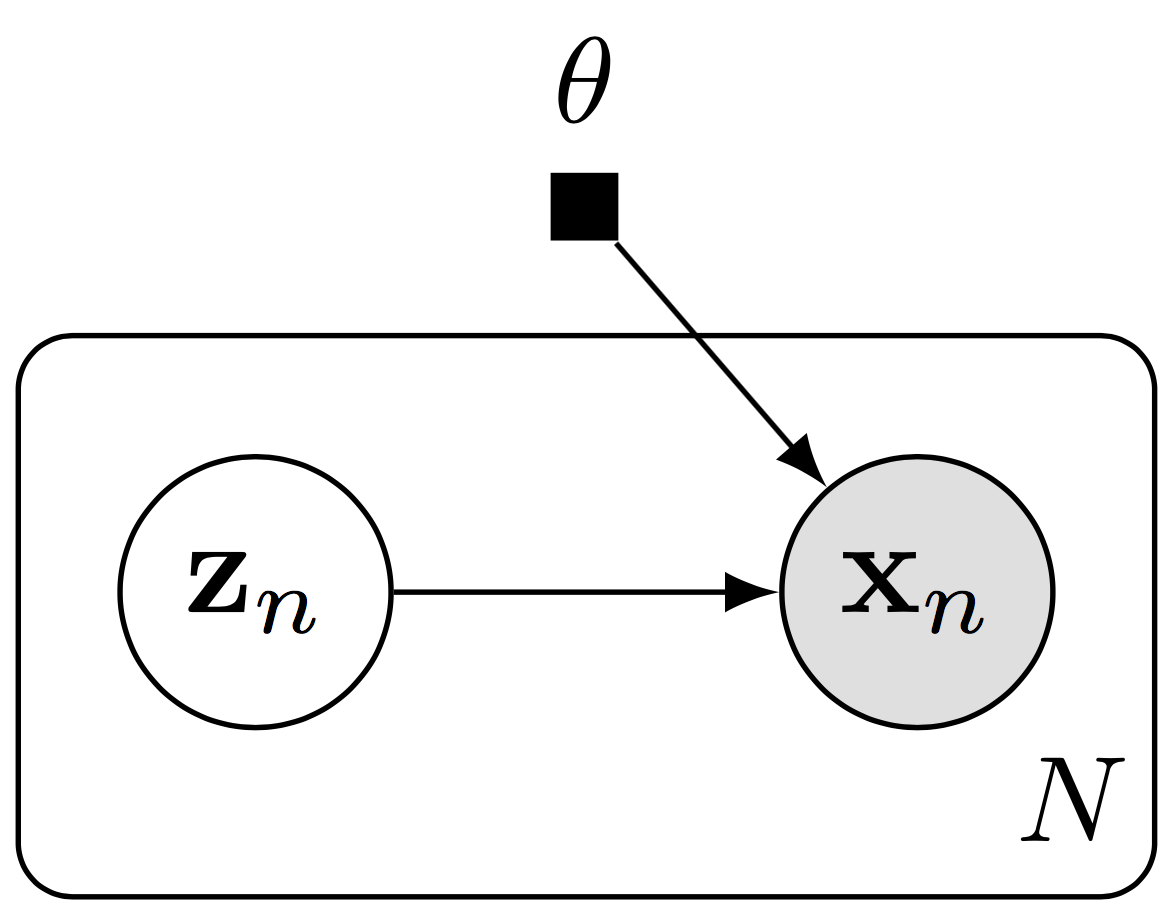
\includegraphics[width=250px]{/images/decoder.png}

{\small\textit{Graphical model of a probabilistic decoder, with model
parameters $\theta$.}}

For real-valued data,
the randomness in the decoder is given by a multivariate Gaussian
\begin{align*}
  p(\mathbf{x}_n\mid\mathbf{z}_n)
  &=
  \text{Normal}(\mathbf{x}_n\mid [\mu,\sigma^2]=\mathrm{NN}(\mathbf{z}_n; \mathbf{\theta})),
\end{align*}
where the probabilistic decoder is parameterized by a neural network
$\mathrm{NN}$ taking the code $\mathbf{z}_n$ as input.

For binary data,
the randomness in the decoder is given by a Bernoulli
\begin{align*}
  p(\mathbf{x}_n\mid\mathbf{z}_n)
  &=
  \text{Bernoulli}(\mathbf{x}_n\mid p=\mathrm{NN}(\mathbf{z}_n; \mathbf{\theta})).
\end{align*}
Probabilistic decoders are typically used alongside a standard normal
prior over the code
\begin{align*}
  p(\mathbf{z})
  &=
  \text{Normal}(\mathbf{z} \mid \mathbf{0}, \mathbf{I}).
\end{align*}

Let's build the model in Edward using
Keras as an easy way to build neural networks. Here we use a
probabilistic decoder to model binarized 28 x 28
pixel images from MNIST.
\begin{lstlisting}[language=Python]
from edward.models import Bernoulli, Normal
from keras.layers import Dense

z = Normal(mu=tf.zeros([N, d]), sigma=tf.ones([N, d]))
hidden = Dense(256, activation='relu')(z)
x = Bernoulli(logits=Dense(28 * 28)(hidden))
\end{lstlisting}
It starts with a $d$-dimensional standard normal prior, one for each
data point. Then it applies a layer of 256 hidden units with
\texttt{relu} nonlinearity. The output layer is $28\cdot 28$ units
without a nonlinearity. This output
parameterizes the Bernoulli's logits. Logits are a more numerically stable
parameterization than probabilities constrained
from 0 and 1.

An example script using this model can be found at
\href{https://github.com/blei-lab/edward/blob/master/examples/vae.py}
{\texttt{examples/vae.py}} in the Github repository.
An example with a convolutional architecture can be found at
\href{https://github.com/blei-lab/edward/blob/master/examples/vae_convolutional_prettytensor.py}
{\texttt{examples/vae_convolutional_prettytensor.py}} in the Github repository.
%We experiment with this model in the
%\href{/tutorials/variational-autoencoder}{variational auto-encoder} tutorial.

\subsubsection{Footnotes}

The neural network which parameterizes the probabilistic decoder is
also known as a generative network. It is in analogy to an
\href{/tutorials/inference-networks}{inference network}, which
can parameterize a variational model used for inference,
interpreted as a probabilistic encoder.

Traditionally, a probabilistic encoder is the most common
choice of inference. This lead to the coinage of the model-inference
combination known as the variational auto-encoder
\citep{kingma2014auto}, which is a probabilistic extension of
auto-encoders.
We recommend against this terminology,
in favor of making explicit the separation of model and inference.
That is, probabilistic decoders are a general class of
models that can be used without an encoder.
Variational
inference is not necessary to infer probabilistic decoders, and
variational inference can also be done without an inference network.

\subsubsection{References}\label{references}

